% Optional figure snippets. Requires graphicx. Figures 03 and 06 are best at landscape width.
% The included PDFs embed their fonts. These snippets are not inserted into main.tex.

\begin{figure}[htbp]
  \centering
  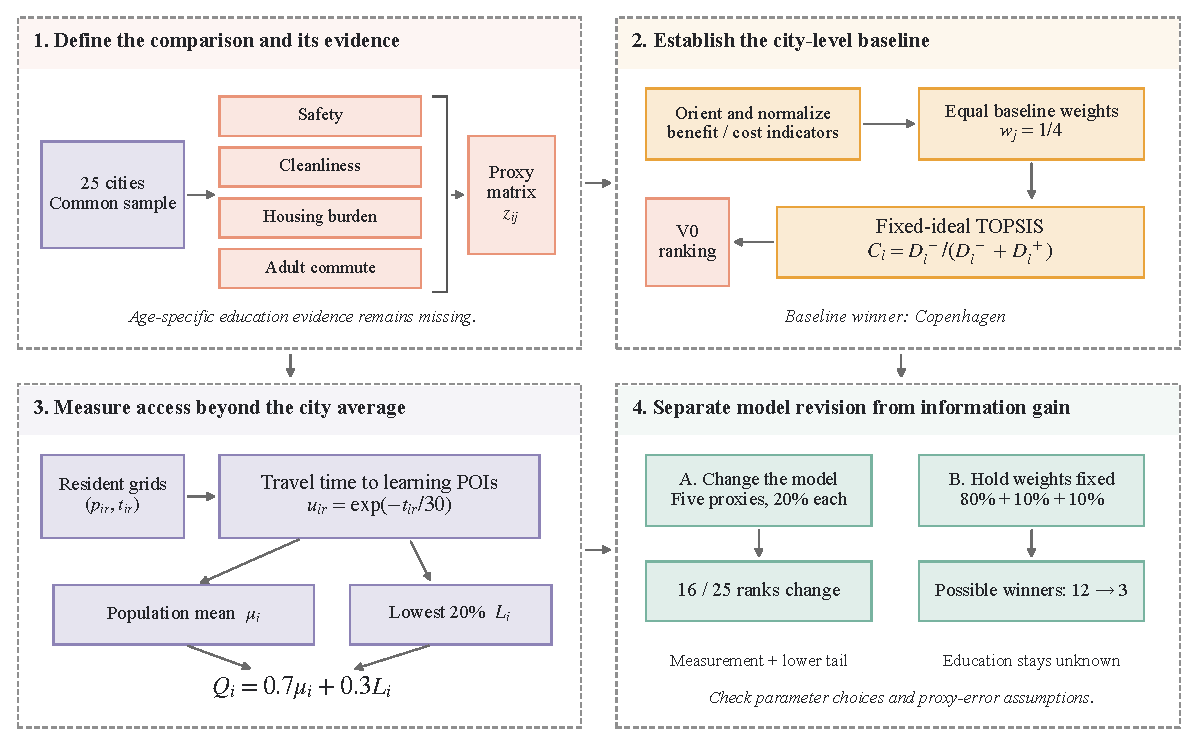
\includegraphics[width=\textwidth]{figures/01_framework.pdf}
  \caption{Model construction and revision. The two experiments in Panel 4 answer different questions; the accessibility proxy does not measure high-school quality or admission eligibility.}
  \label{fig:revision-01-framework}
\end{figure}

\begin{figure}[htbp]
  \centering
  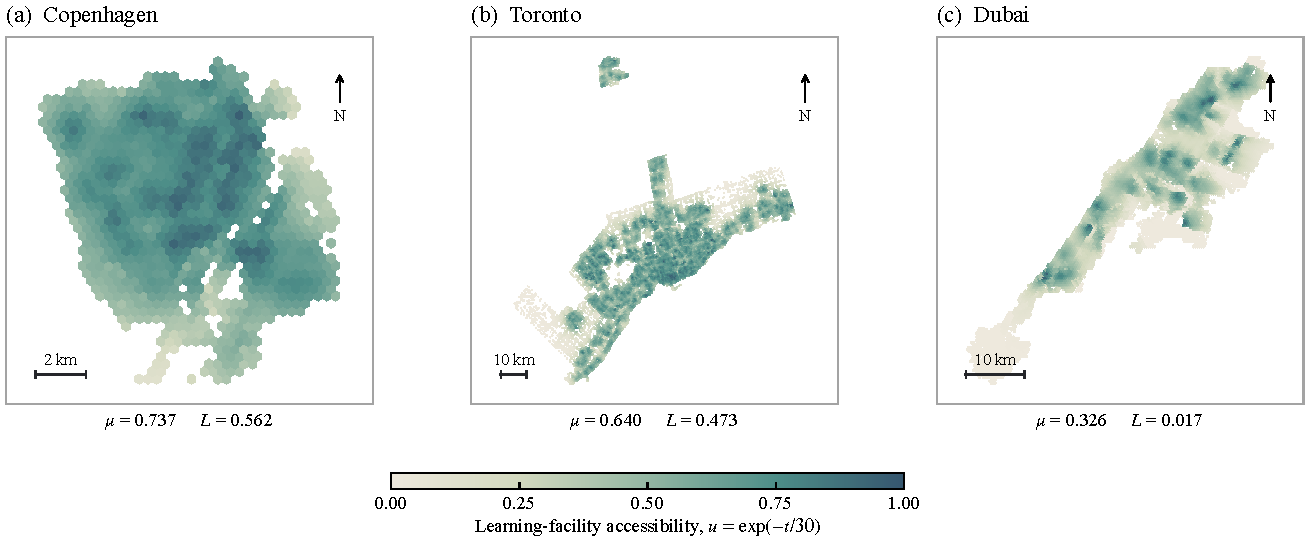
\includegraphics[width=\textwidth]{figures/02_spatial_access.pdf}
  \caption{Learning-facility accessibility in three illustrative cities. Each populated source grid is coloured by model utility. Blank space is outside retained populated grids, not necessarily water or missing facilities. Panel extents differ; local distance conversion and scale bars are approximate. Cases illustrate a stable leader (Copenhagen), upward revision (Toronto) and downward revision (Dubai), not a representative city sample.}
  \label{fig:revision-02-spatial-access}
\end{figure}

\begin{figure}[htbp]
  \centering
  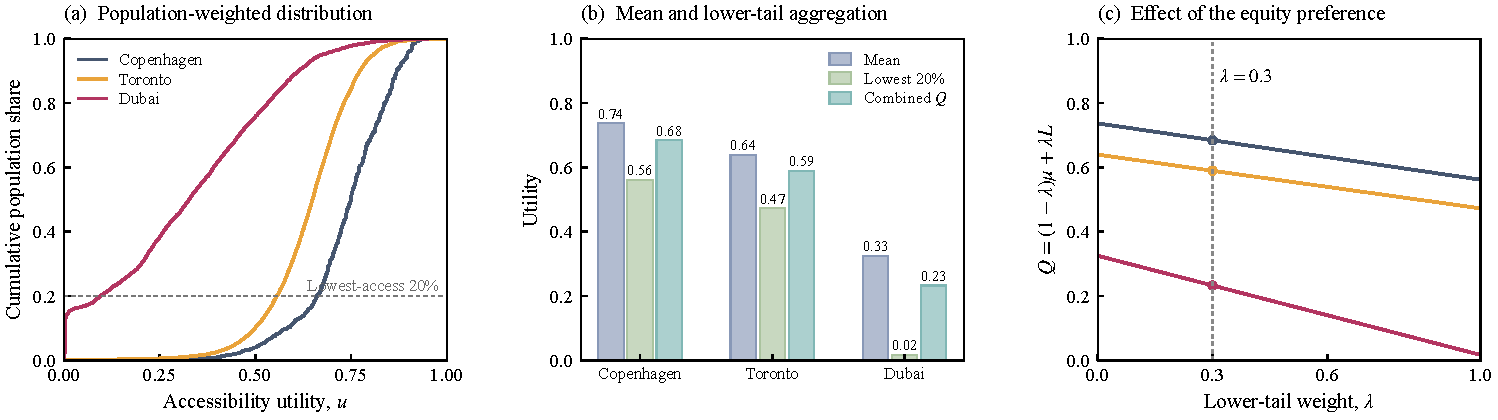
\includegraphics[width=\textwidth]{figures/03_access_mechanism.pdf}
  \caption{Accessibility distributions and the lower-tail mechanism for three illustrative cities. Distributions are weighted by retained all-age population. Panel (c) varies only the normative lower-tail weight; the curves are not fitted empirical relationships. All plotted statistics were checked against the archived analysis.}
  \label{fig:revision-03-access-mechanism}
\end{figure}

\begin{figure}[htbp]
  \centering
  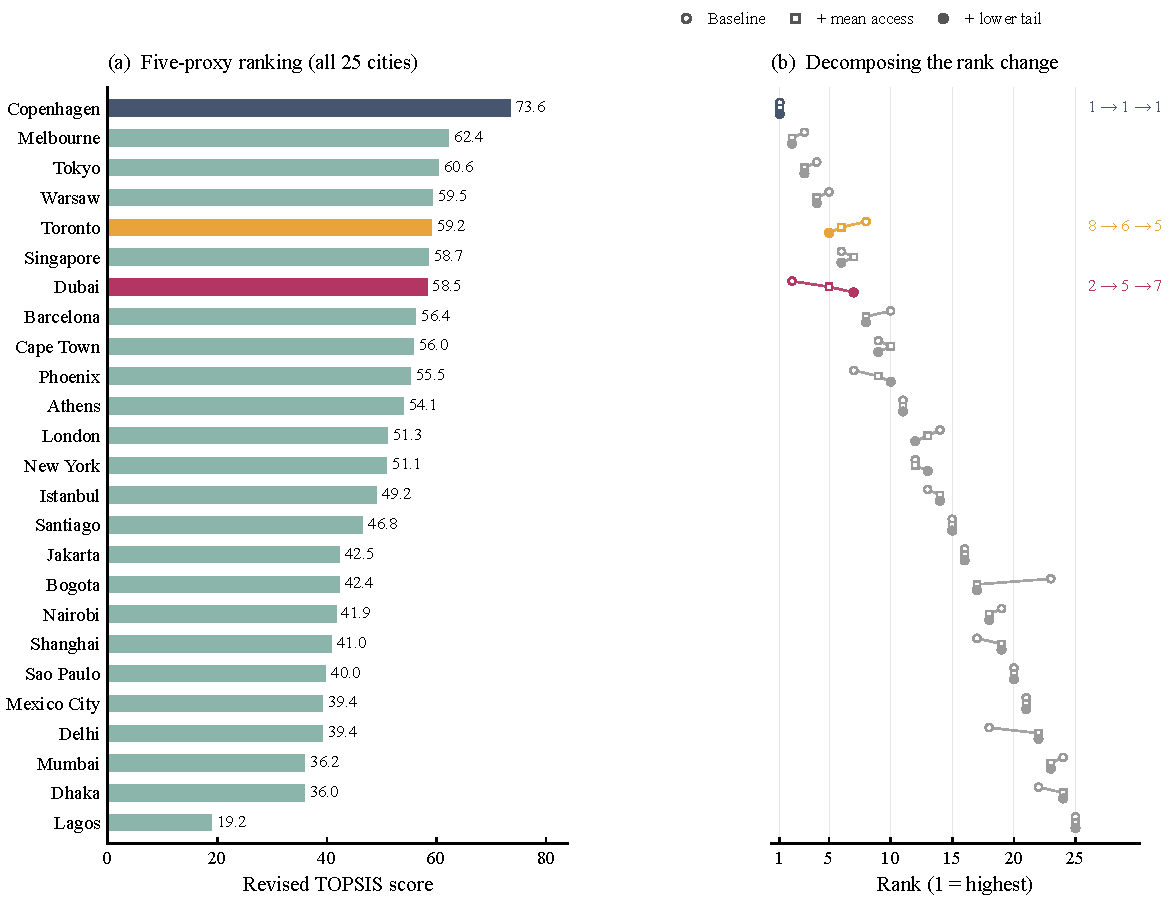
\includegraphics[width=\textwidth]{figures/04_city_ranking.pdf}
  \caption{Conditional ranking under the five-proxy model, with all 25 cities shown. Panel (b) separates the baseline, the addition of mean learning accessibility, and the lower-tail adjustment; vertical offsets separate the three markers for each city and carry no numerical meaning. Score changes across different models are not improvements in city conditions.}
  \label{fig:revision-04-city-ranking}
\end{figure}

\begin{figure}[htbp]
  \centering
  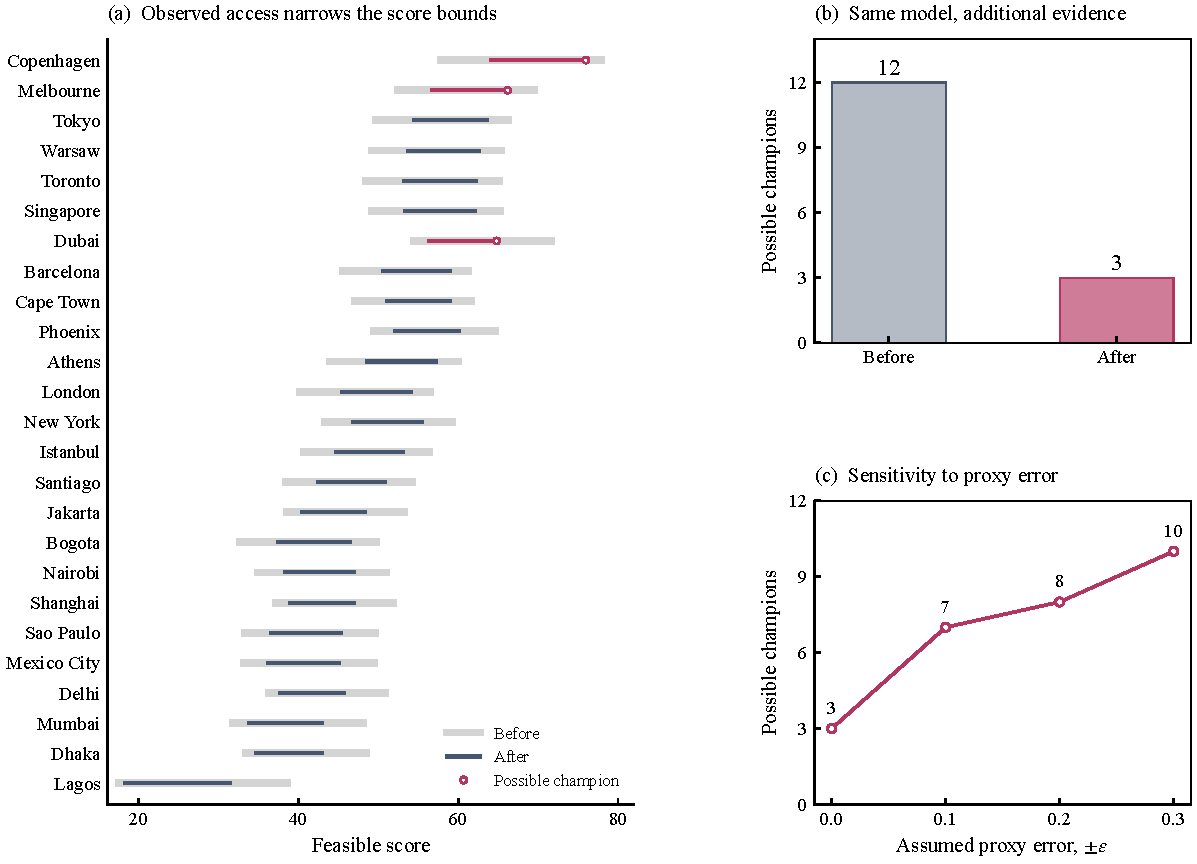
\includegraphics[width=\textwidth]{figures/05_evidence_uncertainty.pdf}
  \caption{Information gain under fixed weights: baseline proxies 80\%, learning accessibility 10\%, unobserved education 10\%. Intervals are feasible bounds, not confidence intervals. The three possible champions after observation are Copenhagen, Dubai and Melbourne. Additional proxy-error widths are stress assumptions, not estimated errors.}
  \label{fig:revision-05-evidence-uncertainty}
\end{figure}

\begin{figure}[htbp]
  \centering
  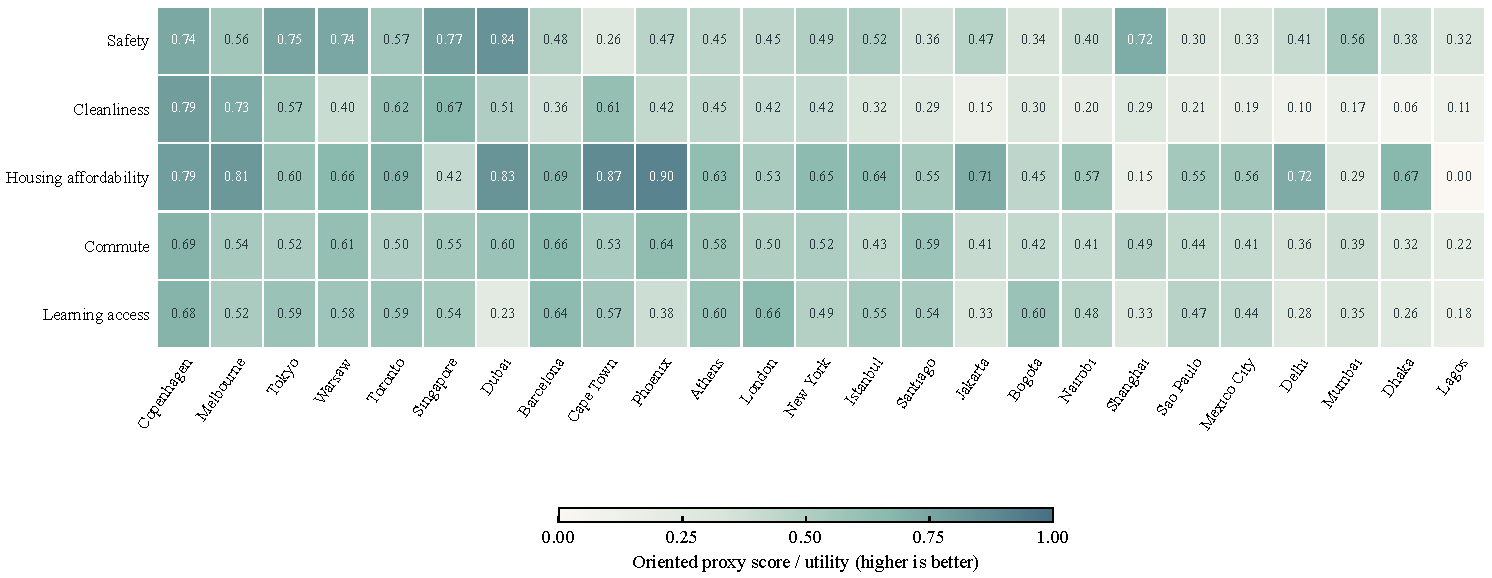
\includegraphics[width=\textwidth]{figures/06_indicator_matrix.pdf}
  \caption{Five proxy indicators for all 25 cities, ordered by the revised ranking. Columns retain every city; the scale is bounded from zero to one. These are oriented proxy scores, not measurements of student outcomes.}
  \label{fig:revision-06-indicator-matrix}
\end{figure}
